 %% ----------------------------------------------------------------
%% Thesis.tex -- MAIN FILE (the one that you compile with LaTeX)
%% ---------------------------------------------------------------- 

% Set up the document
\documentclass[a4paper, 11pt, oneside]{Thesis}  % Use the "Thesis" style, based on the ECS Thesis style by Steve Gunn
\graphicspath{Figures/}  % Location of the graphics files (set up for graphics to be in PDF format)
\usepackage{subcaption}
\usepackage{amsmath,amssymb}

\DeclareRobustCommand{\bbone}{\text{\usefont{U}{bbold}{m}{n}1}}

\DeclareMathOperator{\E}{\mathbb{E}}% expected value
% Include any extra LaTeX packages required
\usepackage[square, numbers, comma, sort&compress]{natbib}  % Use the "Natbib" style for the references in the Bibliography
\usepackage{verbatim}  % Needed for the "comment" environment to make LaTeX comments
\usepackage{vector}  % Allows "\bvec{}" and "\buvec{}" for "blackboard" style bold vectors in maths
\usepackage[toc,page]{appendix}
\hypersetup{urlcolor=blue, colorlinks=true}  % Colours hyperlinks in blue, but this can be distracting if there are many links.
\usepackage{tikz} %flow diagram
\usetikzlibrary{positioning,arrows.meta} %tikz library
\tikzstyle{process} = [rectangle, minimum width=1.2cm, minimum height=1cm, text centered, draw=black, fill=orange!30]
\definecolor{arrowblue}{RGB}{98,145,224}

\newcommand\ImageNode[3][]{
  \node[draw=arrowblue!80!black,line width=1pt,#1] (#2) {\includegraphics[width=2.4cm,height=2.4cm]{#3}};
}

%% ----------------------------------------------------------------
\begin{document}
\frontmatter      % Begin Roman style (i, ii, iii, iv...) page numbering

% Set up the Title Page
\title  {Cartoon-to-real: An Approach to Translate Cartoon to Realistic Images using GAN}
\authors  {\texorpdfstring
            {\href{your web site or email address}{15.01.04.147: Labiba Kanij Rupty\\15.01.04.111: Arefeen Sultan\\15.01.04.127: Nahid Pranto\\15.01.04.133: Sayed Khan Shuvo}}
            {\href{your web site or email address}{Labiba Kanij}}
            }
\addresses  {\groupname\\\deptname\\\univname}  % Do not change this here, instead these must be set in the "Thesis.cls" file, please look through it instead
\date       {\today}
\subject    {}
\keywords   {}

\maketitle
%% ----------------------------------------------------------------

\setstretch{1.3}  % It is better to have smaller font and larger line spacing than the other way round

% Define the page headers using the FancyHdr package and set up for one-sided printing
\fancyhead{}  % Clears all page headers and footers
\rhead{\thepage}  % Sets the right side header to show the page number
\lhead{}  % Clears the left side page header

\pagestyle{fancy}  % Finally, use the "fancy" page style to implement the FancyHdr headers

%% ----------------------------------------------------------------
% Declaration Page required for the Thesis, your institution may give you a different text to place here
 % Declaration ended, now start a new page

%% ----------------------------------------------------------------
% The "Funny Quote Page"
\pagestyle{empty}  % No headers or footers for the following pages

% Now comes the "Funny Quote", written in italics

% The Abstract Page
\addtotoc{Abstract}  % Add the "Abstract" page entry to the Contents
\abstract{
\addtocontents{toc}{\vspace{1em}}  % Add a gap in the Contents, for aesthetics
We show some works to translate cartoon images to real world images using Generative Adversarial Network(GAN). Existing GAN-based image-to-image translation methods which are trained on paired datasets are impractical as the data is difficult to accumulate. Therefore, in this paper we exploit the ideas of \textit{cycle-consistency} and \textit{shared-latent space assumption} method for image translation which needs an unpaired dataset. By applying these methods using different framework(CycleGAN,UNIT,SingleGAN) we compare and show that our model is able to generate meaningful real world images from cartoon images.
}

\clearpage  % Abstract ended, start a new page
%% ----------------------------------------------------------------

\setstretch{1.3}  % Reset the line-spacing to 1.3 for body text (if it has changed)

% The Acknowledgements page, for thanking everyone

% End of the Acknowledgements
%% ----------------------------------------------------------------

\pagestyle{fancy}  %The page style headers have been "empty" all this time, now use the "fancy" headers as defined before to bring them back


%% ----------------------------------------------------------------
\lhead{\emph{Contents}}  % Set the left side page header to "Contents"
\tableofcontents  % Write out the Table of Contents

%% ----------------------------------------------------------------
\lhead{\emph{List of Figures}}  % Set the left side page header to "List if Figures"
\listoffigures  % Write out the List of Figures

%% ----------------------------------------------------------------
\lhead{\emph{List of Tables}}  % Set the left side page header to "List of Tables"
\listoftables  % Write out the List of Tables

%% ----------------------------------------------------------------

\setstretch{1.5}  % Set the line spacing to 1.5, this makes the following tables easier to read
\clearpage  % Start a new page


%% ----------------------------------------------------------------


%% ----------------------------------------------------------------

%% ----------------------------------------------------------------
% End of the pre-able, contents and lists of things
% Begin the Dedication page



%% ----------------------------------------------------------------
\mainmatter	  % Begin normal, numeric (1,2,3...) page numbering
\pagestyle{fancy}  % Return the page headers back to the "fancy" style

% Include the chapters of the thesis, as separate files
% Just uncomment the lines as you write the chapters

\chapter{Introduction}
Many computer vision problems can be considered as an image-to-image translation problem, mapping an image from one domain to another. For example, colorization \cite{DBLP:journals/corr/LarssonMS16} \cite{DBLP:journals/corr/ZhangIE16} (grayscale $\rightarrow$ color), super resolution \cite{DBLP:journals/corr/LedigTHCATTWS16} \cite{DBLP:journals/corr/LaiHA017} (low resolution $\rightarrow$ high resolution), and style transfer \cite{DBLP:journals/corr/GatysEB15a} \cite{DBLP:journals/corr/LiW16} \cite{DBLP:journals/corr/LiaoYYHK17} (image $\rightarrow$ style image). \\
Gatys et al.\cite{DBLP:journals/corr/GatysEB15a} proposed artistic style transfer in his work. By using convolutional neural networks, the author translated any input image into the style of a painting image. Later many works were done in image-to-image translation tasks e.g.\cite{DBLP:journals/corr/LiW16} \cite{DBLP:journals/corr/LiaoYYHK17} where most of them used convolutional neural networks to do the synthesis.\\
Later, Generative Adversarial Network(GAN)\cite{goodfellow2014generative} was proposed which provided astounding results in many tasks, e.g, image generation \cite{DBLP:journals/corr/RadfordMC15} \cite{DBLP:journals/corr/DentonCSF15}, image editing\cite{DBLP:journals/corr/ZhuKSE16}, text2image\cite{DBLP:journals/corr/ZhangXLZHWM16}, image inpainting\cite{DBLP:journals/corr/PathakKDDE16}, image-to-image translation tasks\cite{cyclegan} \cite{pix2pix} etc. Isola et al.\cite{pix2pix} proposed a GAN based approach to transfer input of one domain,$x$ to another domain,$y$ by training on paired image dataset. But accumulating such paired images of both domains is hard and ineffective. We might not get paired images to train for many specific tasks of image-to-image translation. Recently, for training unpaired images, where there is no correspondence between domain $x$ and domain $y$ images, many authors published incredible works such as, CycleGAN\cite{cyclegan}, DualGAN\cite{DBLP:journals/corr/YiZTG17}, DiscoGAN \cite{DBLP:journals/corr/KimCKLK17}, UNIT\cite{DBLP:journals/corr/LiuBK17} etc.\\ 
In unsupervised setting, adversarial loss alone can't solve the infinite mapping problem in the target domain. Zhu et al.\cite{cyclegan} proposed that, by using cycle consistency loss, the network would be able generate images where the possible infinite mappings of target domain would be reduced.\\
Similar work was proposed in UNIT\cite{DBLP:journals/corr/LiuBK17}, where the space-latent assumption implied that the two corresponding sets of different domains can be mapped to a same latent representation in a shared-latent space. To exploit this assumption, the authors proposed a framework based on generative adversarial network(GAN) and variational autoencoders(VAEs).\\
The authors in CartoonGAN\cite{cartoonGAN} paper made an approach in cartoon stylization, transferring a set of real world images to cartoon domain. For this approach, no pairing was required during the training. In this paper, we work on - \textit{Cartoon-to-Real} image translation task. During the training procedure, no pairing of images was required. We extracted cartoon images from different cartoon movies and real images from internet, i.e. flickr. Using our Cartoon-to-Real, we achieve significant result in translating the cartoon images to realistic ones.   

\section{Problem domain}
In recent times, there have been many works on remaking cartoon movies into real live action films e.g. \textit{The Lion King(2019)}, \textit{Beauty and the Beast(2017)} etc. Translating the cartoon images into real world images is a tedious and tiresome work for the film industry. Meanwhile, existing image editing software/algorithms is more costly for bringing CGI effects into films. Therefore, techniques that can automatically transform cartoon images into real world images are very helpful and tremendous amount of time can be saved. Tools such as this also provide as an additional component in photoshop and image editing works. \\
In our work, we do this translation of cartoon images into real world images. For doing this task, we did not need any pairing between two sets of images, cartoon and real world images. We exploited the ideas of cycle consistency\cite{cyclegan} and shared-latent space assumption\cite{DBLP:journals/corr/LiuBK17} and provided effective results in cartoon-to-real images translation.  

\section{Motivation}
CartoonGAN\cite{cartoonGAN} paper proposed a GAN based approach on transforming real world images in cartoon domain. We became interested to transfer the opposite of CartoonGAN, that is, transforming cartoon images to real world images. We see that, many recent movies of cartoons is being made live action film so we were interested in such domain.
\subsection{Why GAN}
Generative adversarial networks provide state of the art results in image-to-image translation tasks. Recently CycleGAN\cite{cyclegan}, UNIT\cite{DBLP:journals/corr/LiuBK17}, SingleGAN\cite{SingleGAN} provides astounding results in this domain. CycleGAN exploits the concept of \textit{cycle consistency loss} where the infinite mappings between two domains is reduced. Similar to \textit{cycle consistency loss} UNIT\cite{DBLP:journals/corr/LiuBK17} proposed another assumption known as shared latent space, where both domains have same shared latent representation. These GAN based approaches provides more effective and efficient results than any other approaches.
 
\section{Contribution}
We implemented cartoon to real world images using Generative Adversarial Network on our unpaired image dataset. For the cartoon domain, we've collected almost 3.1K images scrapped from various movies, e.g. \textit{Pokemon}, \textit{My Neigbour Totoro} and \textit{Kiki’s Delivery}. We used flickr dataset for the real images’ domain. Images are resized to 128×128 resolution. These images,real and cartoon domain images, have no correlations between them We achieved significant results in translating the cartoon images to realistic ones.  % Introduction

\chapter{Background \& Related Work}


\section{Generative Adversarial Networks} \label{GAN}
Generative Adversarial Network(GANs)\cite{goodfellow2014generative} has become a global phenomenon in deep learning algorithms. The algorithm uses two networks, Generators and Discriminators, in a minimax algorithm situation where both of them tries to outperform another in a significant task e.g. image generation \cite{DBLP:journals/corr/RadfordMC15} \cite{DBLP:journals/corr/DentonCSF15}, image editing\cite{DBLP:journals/corr/ZhuKSE16}, text2image\cite{DBLP:journals/corr/ZhangXLZHWM16}, image inpainting\cite{DBLP:journals/corr/PathakKDDE16}, image-to-image translation tasks\cite{cyclegan} \cite{pix2pix} etc. Full objective of GAN function is:
\begin{align}
\min_G \max_D V(D, G)=\mathbb{E}_{x\sim p_{data}(x)}[\log D(x)] + \mathbb{E}_{z\sim p_z(z)}[\log(1 - D(G(z)))]
\end{align}
where Generator G tries to generate images, whereas discriminator D discriminates the output whether it is fake or real. In the objective function, Generator tries to maximize the value of $D(G(z))$ such that it can fool the discriminator,and thus the gap betwen real and fake becomes minimum. The discriminator tries to maximize the term of $[logD(x)]$ and for the 2nd term of $[log(1-D(G(z))]$, discriminator tries to minimize it to 0, which means that the discriminator tries to recognize if the image is generated or real.
\section{Image-To-Image Translation}
Recently, GAN based approach has given tremendous results in image-to-image translation tasks. CycleGAN\cite{cyclegan} proposed a cycle consistency loss to reduce the infinite mappings of input images to any distribution in the target domain. Adversarial loss alone can't solve the random permutation mappings of target distribution, rather it helps the input image to be translated into target domain.\\
In UNIT\cite{DBLP:journals/corr/LiuBK17} framework, the authors proposed a shared-latent space assumption, which denotes that the pair of corresponding images in different domains can be mapped to a same latent representation in a shared-latent space. By using the combination of generative adversarial network(GAN) and variational autoencoders(VAEs) the authors achieved great results in image-to-image translation tasks.
In SingleGAN\cite{SingleGAN} framework, the authors used \textit{cycle consistency loss} \cite{cyclegan}, where one generator is needed instead of using two generators\cite{cyclegan}.  The authors were able to achieve significant results in single domain and multi domain translation. 


\section{Baseline Models}
\subsection{CycleGAN}

While many researchers have produced groundbreaking results such as \cite{pix2pix} ,\cite{sketch-color}, \cite{outdoor} on image-to-image translation using paired data, there hasn't been much successful research using unpaired data. To resolve this case, CycleGAN \cite{cyclegan} has played an influencial role by presenting an approach which translates one image of domain $X$ to another domain $Y$ without any paired training data. This translation is based on an assumption that if an image, $x_i$ from domain $X$ can generate a new image a new image $y_i$ of another domain $Y$, eventually, the generated image, $y_i$ can be mapped to $X$ by generating a new image $\hat{x}$ where \(x_i = \hat{x}\). To sum up, if $G$ is the generator which translates into domain $Y$ and $F$ is for the next translation, we can write it as following -
\begin{equation} \label{eq:ccl1}
G(x_i) = y_i, where\, x_i \in X, y_i \in Y
\end{equation}
\begin{equation} \label{equ:ccl2}
F(y_i)  = \Hat{x}, where\, \Hat{x} \in X 
\end{equation}
Let's break down the ideas that were used to make it a successful research and discuss them one by one.

\subsubsection{Adversarial Loss for CycleGAN} \label{cyc_adv}
Previously, we have known about \textit{Goodfellow et al.}\cite{goodfellow2014generative}  and how it has revolutionized the future of AI. As mentioned in section \ref{GAN}, we know that GAN\cite{goodfellow2014generative} architecture works are based on \textit{Adversarial Loss} which is just an extension of \textit{Binary Cross-Entropy Loss} [Appendix \ref{appendix:BCE}]. However, in the case of CycleGAN\cite{cyclegan}, although \textit{Adversarial Loss} has been used, \textit{Binary Cross Entropy Loss} is not used. The reason is more related to the training inconsistency of GAN\cite{goodfellow2014generative}. From \textit{Mao et al.}, it is known that using \textit{Least Squares Loss} [Appendix \ref{appendix:L2}] shows more stability in training for CycleGAN\cite{cyclegan} than using \textit{Binary Cross-Entropy Loss}. So, equation \ref{eq:adv_loss} of Adversarial loss turns into the following equation, where $c$ is an image from domain $C$ and $r$ from $R$:
    $$ For\, Generator\, G, L_{adv} = \frac{1}{m} \sum^m_{i=1}(1-D_r(G(c)))^2$$
    $$ For\, Generator\, F, L_{adv_cyc} = \frac{1}{m} \sum^m_{i=1}(1-D_c(F(r)))^2$$
However, using only \textit{Adversarial Loss} is not enough to get the best result. This loss is \textit{under-constraint} as it only limits the output to be of a specific domain and fails to limit a closely related output with respect to input. From fig \ref{fig:example}, we can see its demostration. The researchers of CycleGAN\cite{cyclegan} uses an addition loss \textit{Cycle Consitency Loss} to limit the output to be closely related to the input.

\subsubsection{Cycle Consistency Loss} \label{cyc_ccl}
%Cycle Consistency Loss
\begin{figure}[ht]
\begin{center}
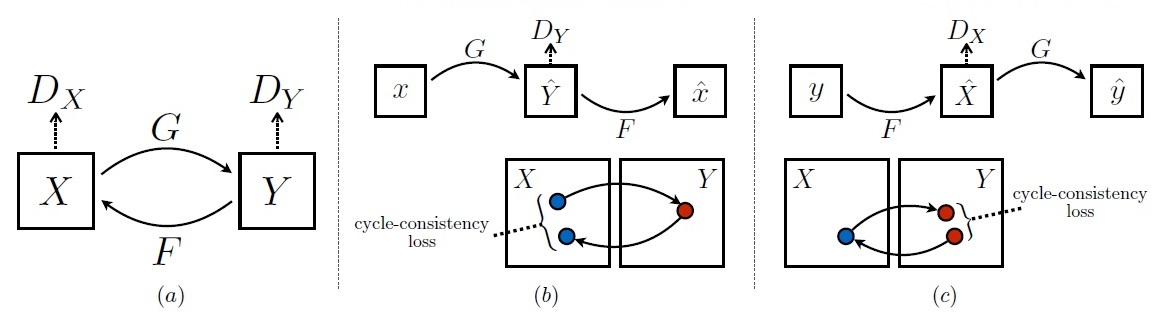
\includegraphics[width=5in,height=2in]{pic/fig3/fig3.jpg}
\caption{Two Mapping Functions with Cycle Consistency Loss in CycleGAN}
\end{center}
\label{fig:ccl_arch}
\end{figure}

The idea of \textit{Cycle Consistency} goes way back. It is an idea of determining the transitivity of two images where second image is the reconstruction of the first image. This transitivity is here denoted as \textit{Loss} in our case, where we use two \textit{Cycle Consistency Loss} as \textit{Forward \& Backward Cycle Consistency Loss}.\\
For our \textit{Cartoon-to-real} translation, if image, $c$ of domain $C$ is to be translated into domain $R$, through \textit{Generator} $G$, there must be another \textit{Generator} $F$ to translate the newly translated image $G(c)$ into $\hat{c}$ with a view to reconstructing $c$. From figure \ref{fig:ccl_arch}, if this \textit{Cycle Consistency Loss} is called \textit{Forward - Cycle Consistency Loss}, the opposite is called \textit{Backward - Cycle Consistency Loss}. It is defined using the following equations -
$$Forward\, Consistency\, Loss, L_{f\_cyc} = \frac{1}{m} \sum^m_{i=1}(F(G(c)) - c) $$
$$Backward\, Consistency\, Loss, L_{b\_cyc} = \frac{1}{m} \sum^m_{i=1}(G(F(r)) - r) $$
\\
A question may arise on why using \textit{Cycle Consistency Loss} solves the \textit{under-constraint} issue. 
\begin{figure}[!ht] 
 \begin{center}
\begin{tikzpicture}[
  node distance=0.8cm,
  >={Triangle[angle=60:1pt 2]},
  shorten >= 2pt,
  shorten <= 2pt,
  arrow/.style={
    ->,
    arrowblue,
    line width=2pt
  }
]
\ImageNode[label={90:Real Anime Pic}]{A}{pic/van/re2.png}
\node (B) [process,below of=A,node distance=3cm] {$D_r$};
\node (C) [process, below of=B,node distance = 2cm] {$\hat r$};
\node (D) [process, right of = C, xshift = 0.8cm] {F};
\node (E) [process, left of = C, xshift = -0.8cm] {G};
\node (F) [process, right of = D, xshift = 0.8cm] {$\hat c$};
\node (G) [process, left of = E, xshift = -0.8cm] {c};
\ImageNode[label={-90:Reconstructed},right=of F]{H}{pic/van/re4.png}
\ImageNode[label={-90:Real},left=of G]{I}{pic/van/re1.png}
\ImageNode[label={-90:Generated Anime Pic},below=of C]{I}{pic/van/re3.png}
\draw[arrow]
  (A) -- (B);
\draw[arrow]
  (C) -- (B); 
\draw[arrow]
  (G) -- (E); 
\draw[arrow]
  (E) -- (C);
\draw[arrow]
  (C) -- (D);
\draw[arrow]
  (D) -- (F);
\end{tikzpicture}
\caption{Architecture Of CycleGAN}
\end{center} 
\label{fig:example}
\end{figure}
The intuition is that for a general mapping of two images, \textit{Adversarial Loss} is great. However, it won't be able to specify the best image of the domain which should be mapped to the first image. On the other hand, \textit{Cycle Consistency Loss} can do this job. Let's think of a scenario, where someone wants to translate \textit{a garden image} to \textit{Monet Painting} using GAN. To his surprise, he finds out that when used only \textit{Adversarial Loss}, the machine translates the garden image with a random monet painting, kind of like figure \ref{fig:example} and on the other hand, when used \textit{Cycle Consitency Loss}, it shows the same contents of the garden which seems to be painted by \textit{Monet}. After some time, he finds out that, as \textit{Cycle Consistency Loss} minimizes the reconstruction loss of the image, the machine is bound to choose an image which is pretty similar to the garden image, as its loss must be the least. So, we can say that, \textit{Cycle Consistency Loss} binds the code to find out the best monet painting to be stylized.
\\

So, the total loss is - 
 $$L(G, F, D_c, D_r) = L_{adv} + L_{f\_cyc} + L_{b\_cyc}$$
 
\subsubsection{Network Architecture \& Training}
CycleGAN\cite{cyclegan} network consists of \textit{two}\textbf{ discriminator} networks and \textit{two} \textbf{generator} networks. The \textbf{discriminator} networks are used as \textbf{PathGANs}. Each \textbf{Generator} has \textit{three} sections: \textsc{Encoder, Transformer, Decoder} [Appendix \ref{appendix:En-Dec}]. Let's take a deeper look into the architecture.
\\
According to \textit{Zhao et al.}\cite{DBLP:journals/tci/ZhaoGFK17}, \textit{L1 Loss} performs best for \textit{Low frequency}[Appendix \ref{appendix:freq}] details, such as \textit{color-blotches, general tonal-distribution/contrast}. However, it fails at preserving \textit{High Frequency}[Appendix \ref{appendix:freq}] details, such as \textit{crisp, edge, texture} etc. Due to the use of \textit{L1 Loss} for \textit{Cycle consistency loss}, the model tends to lose its texture and crisp details. To avoid this situation, \textbf{discriminator} network is forced to model \textit{high frequency} structure. As a result, discriminator uses \textbf{PatchGAN} model which works as a fully collected layer checking a $N \times N$ patch of image every time whether that patch real or fake. In the case of CycleGAN, $70 \times 70$ pixel patch has been used. As texture and styles also work over patch, using \textbf{PatchGAN} preserve them. The architecture of \textbf{PatchGAN} is shown in Table \ref{Patch_Disc}.

\begin{table}[htbp]
\caption{PatchGAN Architecture}
\label{Patch_Disc}
\begin{tabular}{ll}
\hline
Layers &Discriminators \\
\hline
\hline
1 & CONV-(N64,K4,S2),  LeakyRelu \\
2 & CONV-(N128,K4,S2), InstanceNorm, LeakyRelu\\
3 & CONV-(N256,K4,S2), InstanceNorm, LeakyRelu\\
4 & CONV-(N512,K4,S2), InstanceNorm, LeakyRelu\\
\hline
\hline

\end{tabular}
\end{table}


We already know that each \textbf{Generator} consists of \textit{three} architectures within itself. When the input is fed into the network, it directly reaches the encoder, which extracts the representation model of the inputs. It has $three$ convolutional layers. After the final layer, it transforms the input into $256$ channels and passes it to the \textit{transformer} architecture. It is composed of a \textit{Residual Block}[Appendix \ref{appendix:resblock}] which has $6$ convolutional layers. The activated inputs are then expanded using \textbf{decoder} which uses $two$ \textit{deconvolutional layer}[Appendix. \ref{appendix:deconv}] to upsample the image and then a convolutional layer with 3 channels to output an \textbf{RGB} image. The architecture is shown in table \ref{gen_cyc}.
\begin{table}[htbp]
\caption{Generator Architecture of CycleGAN}
\label{gen_cyc}
\begin{tabular}{ll}
\hline
Layers &Generators\\
\hline
\hline
1 & CONV-(N64,K7,S1),InstanceNorm,Relu\\
2 & CONV-(N128,K3,S2),InstanceNorm,Relu\\
3 & CONV-(N256,K3,S2),InstanceNorm,Relu\\
4 & residual-(N256,K3)\\
5 & residual-(N256,K3)\\
6 & residual-(N256,K3)\\
7 & residual-(N256,K3)\\
8 & residual-(N256,K3)\\
9 & residual-(N256,K3)\\
10 & DCONV-(N128,K3,S1/2),fractional,strided, InstanceNorm, Relu\\
11 & DCONV-(N64,K3,S1/2),fractional,strided, IstanceNorm, Relu\\
12 & CONV-(N3,K7,S1),InstanceNorm,Relu\\
\hline
\hline
\end{tabular}
\end{table}

GAN has a tendency to show \textit{Mode Collapse}[Appendix \ref{mode_collapse}] which makes training so hard. To avoid \textit{Mode Collapse} in CycleGAN\cite{cyclegan}, last $50$ generated images are kept in a pool to train the discriminator instead of just training with the last generated image. This technique was acquired from \textit{Shrivastava et al.}\cite{DBLP:conf/cvpr/ShrivastavaPTSW17}.
\subsubsection{Limitations}

Although the output of generating cartoon images into real images look realistic, we can see from figure \ref{fig:lim} that, some of the outputs fail to preserve contents. From figure \ref{fig:lab_a}, CycleGAN\cite{cyclegan} outputs a firing sea whereas input image contains only sky. This has been the case for various outputs which is the biggest limitation of CycleGAN\cite{cyclegan} for our project.
\begin{figure}[!tbp]
\hspace{5cm}Input  \hspace{2.2cm} Output
\begin{center}
     \begin{subfigure}
    
         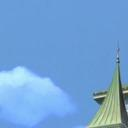
\includegraphics[scale = 0.7]{baaje_pic/Cycle/lat_real.png}
         \label{fig:lab_a}
     \end{subfigure}
     \begin{subfigure}
         
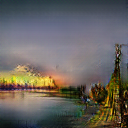
\includegraphics[scale = 0.7]{baaje_pic/Cycle/lat_fake.png}
     \end{subfigure}
\\

     \begin{subfigure}
    
        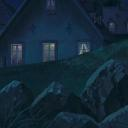
\includegraphics[scale = 0.7]{baaje_pic/Cycle/kds_real.png}
     \end{subfigure}
     \begin{subfigure}
         
        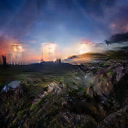
\includegraphics[scale = 0.7]{baaje_pic/Cycle/kdf_fake.png}
     \end{subfigure}
     \caption{Comparison}
\label{fig:lim}
\end{center}
\end{figure}

\subsection{UNIT}
Researchers of UNIT\cite{DBLP:journals/corr/LiuBK17} worked on an assumption known as shared latent space assumption, where a pair of corresponding images in different domains can be mapped to a same latent representation in a shared-latent space. The framework combined a variational autoencoder(VAE) and generative adversarial network (GAN). The adversarial training objective enforces the generator to transform corresponding images in two domains, while the variational autoencoders(VAE) make correlations between translated images with input images in the respective domain.\\ 

\subsubsection{Network Architecture \& Training}
The following abbreviation for ease of presentation is used: N=Neurons, K=Kernel size, S=Stride size. The transposed convolutional layer is denoted as DCONV. The residual basic block is denoted as RESBLK.

\begin{table}[htbp]
\caption{Network Architecture of Encoders and Generators MNIST $\rightarrow$ USPS}
\label{UNIT}
\begin{tabular}{ll}
\hline
Layers & Encoders\\
\hline
\hline
1 & CONV-(N64,K5,S2), BatchNorm, LeakyReLU \\
2 & CONV-(N128,K5,S2), BatchNorm, LeakyReLU \\
3 & CONV-(N256,K8,S1), BatchNorm, LeakyReLU \\
4 & CONV-(N512,K1,S1), BatchNorm, LeakyReLU \\
5 & CONV-(N1024,K1,S1)\\
\hline
Layers & Generators \\
\hline
\hline
1 & DCONV-(N512,K4,S2), BatchNorm, LeakyReLU \\
2 & DCONV-(N256,K4,S2), BatchNorm, LeakyReLU \\
3 & DCONV-(N128,K4,S2), BatchNorm, LeakyReLU \\
4 & DCONV-(N64,K4,S2), BatchNorm, LeakyReLU \\
5 & DCONV-(N3,K1,S1), TanH \\
\hline
\hline

\end{tabular}
\end{table}

\begin{table}[htbp]
\caption{Network Architecture of Discriminators MNIST $\rightarrow$ USPS}
\label{UNIT1}
\begin{tabular}{ll}
\hline
Layers & Discriminators\\
\hline
\hline
1 & CONV-(N20,K5,S1), MaxPooling-(K2,S2) \\
2 & CONV-(N50,K5,S1), MaxPooling-(K2,S2) \\
3 & FC-(N500), ReLU, Dropout \\
4a & FC-(N1), Sigmoid \\
4b & FC-(N10), Softmax \\

\hline
\hline

\end{tabular}
\caption{Network Architecture of Discriminators SVHN $\rightarrow$ MNIST}
\label{UNIT1}
\begin{tabular}{ll}
\hline
Layers & Discriminators\\
\hline
\hline
1 & CONV-(N64,K5,S1), MaxPooling-(K2,S2) \\
2 & CONV-(N128,K5,S1), MaxPooling-(K2,S2) \\
3 & CONV-(N256,K5,S1), MaxPooling-(K2,S2) \\
4 & CONV-(N512,K5,S1), MaxPooling-(K2,S2) \\
5a & FC-(N1), Sigmoid \\
5b & FC-(N10), Softmax \\

\hline
\hline

\end{tabular}

\end{table}

\subsubsection{Limitations}
In UNIT\cite{DBLP:journals/corr/LiuBK17} outputs, the images tend to be soft on the surfaces of the outputs. In real world images, the surfaces are not that smooth as it is in UNIT outputs. Real world images tends to be less sharpen on the edges and more crisp on the surface.  

\begin{figure}
\hspace{5cm}Input  \hspace{2.2cm} Output
\begin{center}
     \begin{subfigure}
    
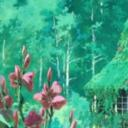
\includegraphics[scale = 0.7]{baaje_pic/UNIT/286_c.jpg}
         \label{fig:ulab_a}
     \end{subfigure}
     \begin{subfigure}
         
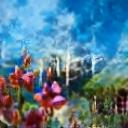
\includegraphics[scale = 0.7]{baaje_pic/UNIT/286_r.jpg}
     \end{subfigure}
\\

     \begin{subfigure}
    
        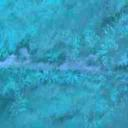
\includegraphics[scale = 0.7]{baaje_pic/UNIT/143_c.jpg}
     \end{subfigure}
     \begin{subfigure}
         
        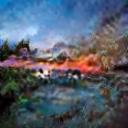
\includegraphics[scale = 0.7]{baaje_pic/UNIT/143_r.jpg}
     \end{subfigure}
     \caption{Comparison}
\label{fig:lim_un}
\end{center}
\end{figure}
\subsection{SingleGAN}
We have already known about two models which consist of multiple generators and discriminators. However, using multiple generators might be ineffective and inefficient. To reduce inefficiency, researchers of SingleGAN \cite{SingleGAN} worked on producing unpaired image translation using a \textbf{Single Generator}. Basically, it is a multi-domain image-to-image translation using \textit{Single Generator} and multiple \textit{Generative Adversarial}  Learning Objects. \\

Intuitively, while translating an image of one domain to another, there exists some common features, such as content, edge of the first domain which will retain its position even after translation. From figure \ref{fig: common}, we get an idea how this works where $3$ of domain 1 and domain 2 share common features which at this point is clearly the edge.
\begin{figure}[!htp] 
\centering
    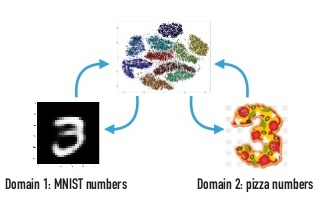
\includegraphics[scale = 1.3]{shared_domain_singleGAN.jpg}
    \caption{In this figure, $3$ of domain $1$(\textit{MNIST Dataset) and pizza-looking $3$ of domain $2$ share common features.}}
\label{fig: common}
\end{figure}
\\
Researchers of singleGAN use this intuition for their work. They generalize the model by sharing these features. For specific domain mapping, an domain distribution, retrieved by auxiliary information, is used . \\
For cartoon to real translation, if the auxiliary information is $Z$, $C$ is cartoon domain and $R$ is real domain, we can define the functions as - 
$$x_C^{fake} = G(x_R, Z_c)$$
$$x_R^{fake} = G(x_C, Z_R)$$

Here, domain code is retrieved using \textit{Central Biasing
Instance Normalization (CBIN)}\cite{chen2016infogan} with the help of auxiliary information.

\subsubsection{Loss Functions}
\textbf{SingleGAN} uses $two$ loss functions. These are \textit{Adversarial Loss} and \textit{Cycle Consistency Loss}.\\
As it gets to use a single generator to translate one image to another, it uses $one$ \textit{Adversarial Loss} for each domain translation. In our case, where we have $two$ domains $C$ and $R$, the loss will be as followiing -
$$L_{adv}(G, D_C) = \E_{x_C}[log(D_C(x_C))] + \E_{x_R, Z_C}[log(1 - D_C(G(x_R, Z_C))]$$
$$L_{adv}(G, D_R) = \E_{x_R}[log(D_R(x_R))] + \E_{x_C, Z_R}[log(1 - D_R(G(x_C, Z_R))]$$
As mentioned in \ref{cyc_adv} and \ref{cyc_ccl}, the same problem may also happen in SingleGAN condition. Due to being \textit{unconstraint}, an additional loss, Cycle Consistency loss is used. For our case, the loss will be -
$$L_{cyc_{sing}} = \E_{x_C}[||x_C - G(G(x_C, Z_R), Z_C)||_1] + \E_{x_R}[||x_R - G(G(x_R, Z_C), Z_R)||_1]$$
So, the final loss is -
$$L = L_{adv}(G, D_C) + L_{adv}(G, D_R) + L_{cyc_{sing}}$$

\subsubsection{Network Architecture \& Training}
Generator G uses the ResNet\cite{DBLP:journals/corr/HeZRS15} structure with an encoder-decoder framework, which contains two stride-2 convolution layers for downsampling, six residual blocks and two stride-2 transposed convolution layers for upsampling. All the normalization layers are replaced except upsampling layers. For the discriminators D, two discriminators\cite{DBLP:journals/corr/IsolaZZE16} are used to discriminate the real and fake images in different scales.

\subsubsection{Limitations}
Unfortunately, of all models, \textbf{SingleGAN} performed the worst. The color scheme of the output is totally faded. We can see examples from \ref{fig:lim_sing}
\begin{figure}[!hb]
\hspace{5cm}Input  \hspace{2.2cm} Output
\begin{center}
     \begin{subfigure}
    
         
\includegraphics[scale = 0.7]{baaje_pic/SingleGAN/image076_D0.jpg}
         \label{fig:labs_a}
     \end{subfigure}
     \begin{subfigure}
         
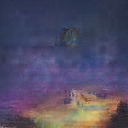
\includegraphics[scale = 0.7]{baaje_pic/SingleGAN/image076_0to1.jpg}
     \end{subfigure}
\\

     \begin{subfigure}
    
        
\includegraphics[scale = 0.7]{baaje_pic/SingleGAN/image259_D0.jpg}
     \end{subfigure}
     \begin{subfigure}
         
        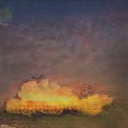
\includegraphics[scale = 0.7]{baaje_pic/SingleGAN/image259_0to1.jpg}
     \end{subfigure}
     \caption{Comparison}
\label{fig:lim_sing}
\end{center}
\end{figure}

 % Background Theory 

\chapter{Progress \& Experiments} \label{chap:prog}
So far, we have studied on CycleGAN\cite{cyclegan}, UNIT\cite{DBLP:journals/corr/LiuBK17} and SingleGAN\cite{SingleGAN} for image-to-image translation tasks. We developed two unpaired datasets to train our network. For the cartoon domain, we've collected almost 3.1K images scrapped from various movies, e.g. \textit{Pokemon}, \textit{My Neigbour Totoro} and \textit{Kiki’s Delivery}. We used flickr dataset for the real images’ domain. Images are resized to 128×128 resolution. For implementation we used PyTorch and for hardware we used Nvidia GTX 1060. We compare our results through different architectures i.e. CycleGAN\cite{cyclegan}, UNIT\cite{DBLP:journals/corr/LiuBK17} and SingleGAN\cite{SingleGAN}.\\
In some images, \textit{cycle consistency loss} was unable to preserve content representation of input image. However, UNIT\cite{DBLP:journals/corr/LiuBK17} was able to maintain content of input image in the output. Still it has some flaws, as UNIT tends to smoothen the surface of output images, where in real world surfaces are tend to be crisp and less sharpen on the edges. In SingleGAN\cite{SingleGAN}, output images colors become faded and the content is not preserved most of the time.

%First Comparison
\begin{figure}[ht]
Input \hspace{2.7cm} CycleGAN \hspace{1.8cm} UNIT \hspace{2.4cm} SingleGAN
\begin{center}
     \begin{subfigure}
    
         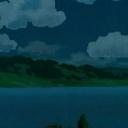
\includegraphics[scale = 0.7]{pic/in/i1.png}
     \end{subfigure}
     \hspace{0.1in}
     \begin{subfigure}
         
         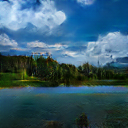
\includegraphics[scale = 0.7]{pic/cgan/c1.png}
     \end{subfigure}
     \hspace{0.1in}
     \begin{subfigure}
         
         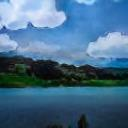
\includegraphics[scale = 0.7]{pic/unit/u1.jpg}
     \end{subfigure}
     \hspace{0.1in}
     \begin{subfigure}
        
         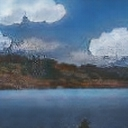
\includegraphics[scale = 0.7]{pic/sgan/s1.jpg}
     \end{subfigure}
     \begin{subfigure}
         
         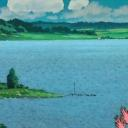
\includegraphics[scale = 0.7]{pic/in/i2.png}
     \end{subfigure}
     \hspace{0.1in}
     \begin{subfigure}
         
         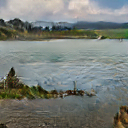
\includegraphics[scale = 0.7]{pic/cgan/c2.png}
     \end{subfigure}
     \hspace{0.1in}
     \begin{subfigure}
         
         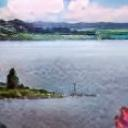
\includegraphics[scale = 0.7]{pic/unit/u2.jpg}
     \end{subfigure}
     \hspace{0.1in}
     \begin{subfigure}
        
         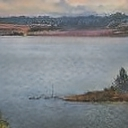
\includegraphics[scale = 0.7]{pic/sgan/s2.jpg}
     \end{subfigure}
     \begin{subfigure}
         
         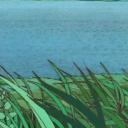
\includegraphics[scale = 0.7]{pic/in/i3.png}
     \end{subfigure}
     \hspace{0.1in}
     \begin{subfigure}
         
         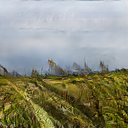
\includegraphics[scale = 0.7]{pic/cgan/c3.png}
     \end{subfigure}
     \hspace{0.1in}
     \begin{subfigure}
         
         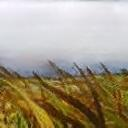
\includegraphics[scale = 0.7]{pic/unit/u3.jpg}
     \end{subfigure}
     \hspace{0.1in}
     \begin{subfigure}
        
         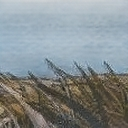
\includegraphics[scale = 0.7]{pic/sgan/s3.jpg}
     \end{subfigure}
     \begin{subfigure}
         
         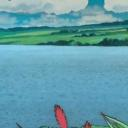
\includegraphics[scale = 0.7]{pic/in/i4.png}
     \end{subfigure}
     \hspace{0.1in}
     \begin{subfigure}
         
         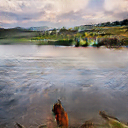
\includegraphics[scale = 0.7]{pic/cgan/c4.png}
     \end{subfigure}
     \hspace{0.1in}
     \begin{subfigure}
         
         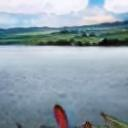
\includegraphics[scale = 0.7]{pic/unit/u4.jpg}
     \end{subfigure}
     \hspace{0.1in}
     \begin{subfigure}
        
         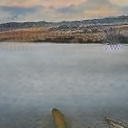
\includegraphics[scale = 0.7]{pic/sgan/s4.jpg}
     \end{subfigure}
     \begin{subfigure}
         
         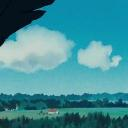
\includegraphics[scale = 0.7]{pic/in/i5.png}
     \end{subfigure}
     \hspace{0.1in}
     \begin{subfigure}
         
         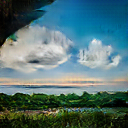
\includegraphics[scale = 0.7]{pic/cgan/c5.png}
     \end{subfigure}
     \hspace{0.1in}
     \begin{subfigure}
         
         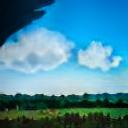
\includegraphics[scale = 0.7]{pic/unit/u5.jpg}
     \end{subfigure}
     \hspace{0.1in}
     \begin{subfigure}
        
         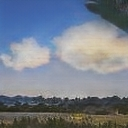
\includegraphics[scale = 0.7]{pic/sgan/s5.jpg}
     \end{subfigure}
     \begin{subfigure}
         
         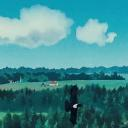
\includegraphics[scale = 0.7]{pic/in/i6.png}
     \end{subfigure}
     \hspace{0.1in}
     \begin{subfigure}
         
         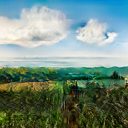
\includegraphics[scale = 0.7]{pic/cgan/c6.png}
     \end{subfigure}
     \hspace{0.1in}
     \begin{subfigure}
         
         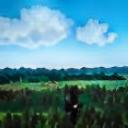
\includegraphics[scale = 0.7]{pic/unit/u6.jpg}
     \end{subfigure}
     \hspace{0.1in}
     \begin{subfigure}
        
         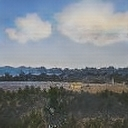
\includegraphics[scale = 0.7]{pic/sgan/s6.jpg}
     \end{subfigure}
     
     \caption{Comparison Between CycleGAN, UNIT and SingleGAN}
     \label{fig:compare1}
\end{center}
\end{figure}

%Second Comparison
\begin{figure}[ht]
Input \hspace{2.7cm} CycleGAN \hspace{1.8cm} UNIT \hspace{2.4cm} SingleGAN
\begin{center}
     \begin{subfigure}
    
         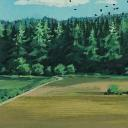
\includegraphics[scale = 0.7]{pic/in/i7.png}
     \end{subfigure}
     \hspace{0.1in}
     \begin{subfigure}
         
         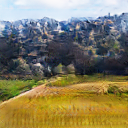
\includegraphics[scale = 0.7]{pic/cgan/c7.png}
     \end{subfigure}
     \hspace{0.1in}
     \begin{subfigure}
         
         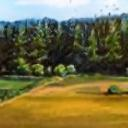
\includegraphics[scale = 0.7]{pic/unit/u7.jpg}
     \end{subfigure}
     \hspace{0.1in}
     \begin{subfigure}
        
         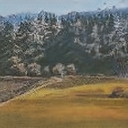
\includegraphics[scale = 0.7]{pic/sgan/s7.jpg}
     \end{subfigure}
     \begin{subfigure}
         
         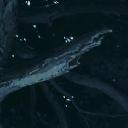
\includegraphics[scale = 0.7]{pic/in/i8.png}
     \end{subfigure}
     \hspace{0.1in}
     \begin{subfigure}
         
         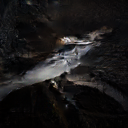
\includegraphics[scale = 0.7]{pic/cgan/c8.png}
     \end{subfigure}
     \hspace{0.1in}
     \begin{subfigure}
         
         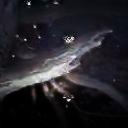
\includegraphics[scale = 0.7]{pic/unit/u8.jpg}
     \end{subfigure}
     \hspace{0.1in}
     \begin{subfigure}
        
         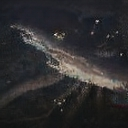
\includegraphics[scale = 0.7]{pic/sgan/s8.jpg}
     \end{subfigure}
     \begin{subfigure}
         
         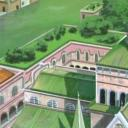
\includegraphics[scale = 0.7]{pic/in/i9.png}
     \end{subfigure}
     \hspace{0.1in}
     \begin{subfigure}
         
         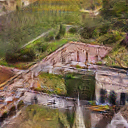
\includegraphics[scale = 0.7]{pic/cgan/c9.png}
     \end{subfigure}
     \hspace{0.1in}
     \begin{subfigure}
         
         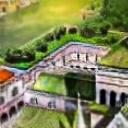
\includegraphics[scale = 0.7]{pic/unit/u9.jpg}
     \end{subfigure}
     \hspace{0.1in}
     \begin{subfigure}
        
         \includegraphics[scale = 0.7]{pic/sgan/s9.jpg}
     \end{subfigure}
     \begin{subfigure}
         
         \includegraphics[scale = 0.7]{pic/in/i10.png}
     \end{subfigure}
     \hspace{0.1in}
     \begin{subfigure}
         
         \includegraphics[scale = 0.7]{pic/cgan/c10.png}
     \end{subfigure}
     \hspace{0.1in}
     \begin{subfigure}
         
         \includegraphics[scale = 0.7]{pic/unit/u10.jpg}
     \end{subfigure}
     \hspace{0.1in}
     \begin{subfigure}
        
         \includegraphics[scale = 0.7]{pic/sgan/s10.jpg}
     \end{subfigure}
     \begin{subfigure}
         
         \includegraphics[scale = 0.7]{pic/in/i11.png}
     \end{subfigure}
     \hspace{0.1in}
     \begin{subfigure}
         
         \includegraphics[scale = 0.7]{pic/cgan/c11.png}
     \end{subfigure}
     \hspace{0.1in}
     \begin{subfigure}
         
         \includegraphics[scale = 0.7]{pic/unit/u11.jpg}
     \end{subfigure}
     \hspace{0.1in}
     \begin{subfigure}
        
         \includegraphics[scale = 0.7]{pic/sgan/s11.jpg}
     \end{subfigure}
     \begin{subfigure}
         
         \includegraphics[scale = 0.7]{pic/in/i12.png}
     \end{subfigure}
     \hspace{0.1in}
     \begin{subfigure}
         
         \includegraphics[scale = 0.7]{pic/cgan/c12.png}
     \end{subfigure}
     \hspace{0.1in}
     \begin{subfigure}
         
         \includegraphics[scale = 0.7]{pic/unit/u12.jpg}
     \end{subfigure}
     \hspace{0.1in}
     \begin{subfigure}
        
         \includegraphics[scale = 0.7]{pic/sgan/s12.jpg}
     \end{subfigure}
     
     \caption{Comparison Between CycleGAN, UNIT and SingleGAN}
     \label{fig:compare2}
\end{center}
\end{figure}

%Data Flow Diagram


 % Experimental Setup


\chapter{Future Plans \& Conclusion}
After the experiments and results we achieved from Chapter \ref{chap:prog}, we noted some observations. Those are described below - \\
From the output of Figure \ref{fig:compare1}, \ref{fig:compare2}, it is seen that \textbf{CycleGAN} gives pretty realistic output. It seems almost real at the first glance. However, after taking a close look from Figure \ref{fig:lim}, we came to conclusion that, the content of the input image is not quite retrieved in \textbf{CycleGAN} outputs. In fact, it translates skies to seas and seas to skies.\\
Again, for \textbf{SingleGAN}, we notice that, this model doesn't produce much satisfactory result. From Figure \ref{fig:lim_sing} and even from \ref{fig:compare1}, \ref{fig:compare2}, we see that \textbf{SingleGAN} doesn't excel at all. The color is too faded and the contents are not retrieved perfectly.\\
Lastly, for \textbf{UNIT}'s case, we see that the model is succeeded in retrieving every pixel of the input perfectly. Almost no output can be seen where it varies too much from input. However, according to Figure \ref{fig:lim_un}, as much perfect content-wise as it is, it fails in making outputs more realistic. They seem pretty cartoonish due to the smoothness of the surface.

\section{Final Decision}

From the above observations, we decided to emphasize more on \textbf{CycleGAN} and \textbf{UNIT} as they complement each other. We are excluding \textbf{SingleGAN} as it fails to produce any output close to our satisfaction. Assuming that making the output sharper will improve the result, we planned $four$ options. These are discussed below -

\subsection{Preprocessing Input}
Previously, we used the raw dataset as our input. As our output lacks sharpness, we assume that adding more crisp in the input might give us a better realistic output. On this case, we want to add more details on \textbf{UNIT} model and see how that impacts our result.
\subsection{Using Sharpening Loss}
Another idea to add more crisp in the output is to use sharpening loss. We got this idea from \textbf{CartoonGAN} \cite{cartoonGAN}. \textbf{CartoonGAN} uses an \textit{edge loss} function to create more cartoonish images as they observed that cartoons tend to have sharper edge than real images. We decided to implement idea on \textbf{UNIT} model. Instead of using edge loss function, we will use \textit{Sharpening Loss} Function.
\subsection{PatchGAN as Discriminator}

We know from Section \ref{cyc_ccl} that, \textbf{CycleGAN} uses \textit{PatchGAN} as discriminator to reduce loss of high frequency details of images such as crisp, texture. We may guess why \textit{CycleGAN} perfroms better in case of high frequency details. So, we decided to add \textbf{PatchGAN} discriminator into \textbf{UNIT} model as an option to improve our result.

\section{Conclusion}
In this report, we have discussed about our topic in-depth. We showed our experiments based on our project. We made a brief overview of the models of the experiments and their architecture and how they work. Finally, we analyzed all these experiments and developed a plan to improve our project. Our goal is to produce a result which will as real as it can get. % Experiment 1



%\input{Chapters/Chapter6} % Results and Discussion

%\input{Chapters/Chapter7} % Conclusion

%% ----------------------------------------------------------------
% Now begin the Appendices, including them as separate files

\addtocontents{toc}{\vspace{2em}} % Add a gap in the Contents, for aesthetics

\appendix % Cue to tell LaTeX that the following 'chapters' are Appendices

\chapter{Appendix A}
\begin{appendices}

\section{Binary Cross Entropy Loss}
\label{appendix:BCE}
A criterion to measure the Binary Cross Entropy between the target and the output. The loss can be described as:\\
    $\ell(x, y) = L = \{l_1,\dots,l_N\}^\top, \quad
l_n = - w_n \left[ y_n \cdot \log x_n + (1 - y_n) \cdot \log (1 - x_n) \right],$\\
where N is the batch size.

\section{Why Least Squares Loss more suitable for GAN}
\label{appendix:L2}
for $\mathcal{L}_{adv}$(Adversarial loss), the negative log likelihood objective is replaced by a least-squares loss. This loss is more stable during training and generates higher quality results.

\section{Encoder - Decoder Network}
\label{appendix:En-Dec}
From \cite{BibEntry2018Nov}, 
“Generally, the encoder encodes the input sequence to an internal representation called 'context vector' which is used by the decoder to generate the output sequence. The lengths of input and output sequences can be different, as there is no explicit one on one relation between the input and output sequences.”
\\
To sum up, an encoder is a network such as \textit{CNN, RNN, MLP}, which extracts a feature vector from raw inputs and then outputs the feature vecor. And decoder is also a network, which takes that output feature vector as input and produces an output which represents the input in the best way possible.
\section{Low \& High Frequency Image}
\label{appendix:freq}
\textit{Frequency} means the rate of change per pixel. \textit{A high frequency} image is the one which keeps changing a its pixel in a high rate. A striped picture which has black and white stripes will have the highest frequency, since $0$ is the lowest pixel and then it changes to $255$ which is the highest within a very short time. Again, \textit{a low frequency} image is the one whose pixel values rarely change. For example, a single colored image will have 0 frequency.
\section{Residual Block}
\label{appendix:resblock}
After convolutional nueural network used by \textit{AlexNET} won the \textbf{ImageNET}, the popularity of \textbf{CNN} started to rise. It was assumed that using more layers give better results. However, using more layers produced another problem, \textit{Vanishing Gradient}. It is when after running of few layers, as it goes deeper, the gradient tends to be $zero$. To avoid this problem, after sometime a new model called \textit{ResNET} was created. The main idea of it is to create blocks for which gradient won't be calculated. So, chance of vanishing gradient is decreased. This blocks are called \textbf{Residual Blocks}.
\section{Deconvolutional Layers}
\label{appendix:deconv}

Deconvolutional layer is a term which is often used to denote a reverse convolution. It is used for image upsampling to get back the original image size. It is done in the following manner - by taking each pixel of the input, multiply them with a $3 \times 3$ kernel to get a weighted output, and then it has to be inserted into the output image. When the outputs overlap, it is summed.
\section{Mode Collapse}
\label{mode_collapse}
One of the common problems of GAN is mode collapse problem. In this problem, the generator produces less diversified samples. So there is a possible chance that the generator is generating similar images without any varieties.
 
\end{appendices}

	% Appendix Title

%\input{Appendices/AppendixB} % Appendix Title

%\input{Appendices/AppendixC} % Appendix Title

\addtocontents{toc}{\vspace{2em}}  % Add a gap in the Contents, for aesthetics
\backmatter

%% ----------------------------------------------------------------
\label{Bibliography}
\lhead{\emph{Bibliography}}  % Change the left side page header to "Bibliography"
\bibliographystyle{unsrtnat}  % Use the "unsrtnat" BibTeX style for formatting the Bibliography
\nocite{*}
\bibliography{Bibliography}  % The references (bibliography) information are stored in the file named "Bibliography.bib"

\end{document}  % The End
%% ----------------------------------------------------------------